\chapter{Introdução}

O Programa de Apoio a Planos de Reestruturação e Expansão das Universidades Federais(REUNI) foi instituído pelo DECRETO Nº 6.096, DE 24 DE ABRIL DE 2007 \todo{como cita isso?} possui como uma de suas diretrizes:

\begin{quote}
I - redução das taxas de evasão, ocupação de vagas ociosas e aumento de vagas de ingresso, especialmente no período noturno;
\end{quote}

Na UFC(Universidade Federal do Ceará), de acordo com o último Anuário estatístico\todo{quando sai o próximo?}, de 2014, ano base 2013, o indicador "Taxa de Sucesso na Graduação", definido como a proporção entre número de discentes diplomados e número de discentes ingressantes da graduação\todo{manual de indicadores do TCU, p.5}, esteve em 2013 com o menor valor desde 2008\ref{img:taxa-de-sucesso-ufc}. Já o indicador "Taxa de sucesso da graduação por curso", em 2013\todo{qual a definição?}, possuiu valor médio igual a 64\% e valor mínimo igual a 6.8\%(Tabela \ref{table:ts_2013}).

\begin{figure}
	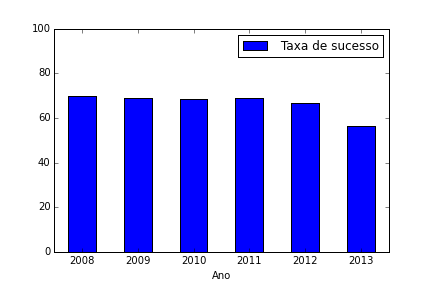
\includegraphics[scale=0.8]{img/taxa-de-sucesso-ufc.png}
	\caption{Taxa de Sucesso na Graduação - UFC}
	\label{img:taxa-de-sucesso-ufc}
\end{figure}

\begin{table}
\begin{tabular}{llc}
\toprule
                            Curso &  Período & Taxa de Sucesso \\
\midrule
  Ciências Sociais - Licenciatura &  Noturno &            6.8\% \\
  Redes de Computadores - Quixadá &  Noturno &           13.3\% \\
          Geografia - Bacharelado &   Diurno &           15.3\% \\
        Letras - Português-Alemão &   Diurno &           17.6\% \\
           Engenharia Metalúrgica &   Diurno &           18.3\% \\
     Ciências Econômicas - Sobral &  Noturno &           20.9\% \\
 Sistemas de Informação - Quixadá &   Diurno &           22.0\% \\
          Filosofia - Bacharelado &  Noturno &           24.3\% \\
         Matemática - Bacharelado &   Diurno &           24.4\% \\
     Engenharia Elétrica - Sobral &   Diurno &           25.0\% \\
\bottomrule
\end{tabular}
\caption{Taxa de sucesso da graduação por curso na UFC em 2013 - 10 piores resultados}
\label{table:ts_2013}
\end{table}

\todo{como resolve}
Uma das estratégias adotadas para diminuir as taxas de evasão é a identificação precoce de discentes com grande tendência para abandonarem seus cursos e a execução de ações que minimizem tal tendência. A identificação pode ser conduzida por observação do comportamento e resultados dos discentes, de forma subjetiva, pelos docentes e coordenadores de cursos, por exemplo. Dois problemas decorrem dessa forma de identificação: sendo conduzida por pessoas, essa forma de identificação é limitada pelo conjunto de observações as quais o observador tem acesso; sendo subjetiva, seus resultados podem sofrer resistência para serem aceitos. A utilização de técnicas de aprendizado de máquina como forma de identificação pode contornar esses problemas, por, primeiro, fazer uso de dados registrados por sistemas de informação, provavelmente contendo informações mais amplas que as que uma pessoa pode observar; segundo, por fazer maior uso de dados registrados, sendo aceita mais facilmente como identificação objetiva. 

Em estudo realizado no departamento de engenharia elétrica da Eindhoven University of Technology\cite{Predicting_Students}, é relatado que em dezembro os discentes desse departamente recebem um aviso informando se são ou não aconselhados a continuarem no curso. Esse aviso é baseado na performance do discente no curso e em informações obtidas de professores do primeiro semestre e de discentes monitores. É relatado que o aviso parece ter bastante acurácia: geralmente discentes aconselhados a continuarem têm sucesso no próximo ano do curso, enquanto aqueles desaconselhados geralmente não continuam no curso. Nesse estudo foram utilizados diversos algoritmos de aprendizado de máquina com o objetivo de tentar detectar que um estudante irá abandonar seu curso. Foram utilizadas informações de discente referentes tanto ao período anterior ao seu ingresso na universidade, quanto ao posterior. \todo{outros estudos}

\todo{dados na ufc}
A UFC possui uma base de dados de informações sobre seus discentes gerada e mantida pelo sistema SIGAA(Sistema Integrado de Gestão de Atividades Acadêmicas)\todo{referencia}

O presente trabalho objetiva avaliar a aplicabilidade de técnicas de mineração de dados sobre o problema de evasão de discentes na UFC a partir dos dados que seus sistemas de informação gerenciam.  

Para tanto é necessário que seja feito uma análise sobre a estrutura e qualidade dos dados disponíveis.

Também serão levantadas hipóteses sobre causas para o problema e será analisado se os dados as corroboram ou não.

hipótese sobre a estrutura do curriculo -> métricas com relação às turmas! por exemplo, distância de horário entre disciplinas do mesmo semestre -> no caso do aluno, para cada semestre calcular

\cite{EDM_brasil}